% -*- mode: latex -*- %

\newcommand{\logit}{\mathop{\rm logit}}

\section{Experiments}
\label{sec:experiments}

%\ha{discuss general goal of this section and what are our hypothesis based on 
%our theoretical analysis.}

%Hypothesis:
%\begin{itemize}
%	\item Non-aggregated MLE is calibrated
%	\item Majority-vote is not calibrated
%	\item Non-aggregated MLE is better for classification
%	\item When we increase $m$, calibration gets worse to majority vote (factor $\sqrt{m}$?)
%	\item When we increase $m$, classification gets better
%	\item When we decrease $\beta$, classification gap is smaller (synthetic experiment)
%\end{itemize}

We conclude the paper with several experiments to 
test the merit of the (sometimes implicit)
methodological suggestions.
%% Before delving into our experimental results, 
We detail a few expected behaviors our theory suggests; if
we fail to see them, then the model we have proposed is too unrealistic to
inform practice.
%
The results
in~\Cref{sec:well-sepcified-mod} suggest the classification error should be
lower for the non-aggregated algorithm $\tmle$, and the gap between
algorithms~\eqref{eq:maximum-likelihood} and~\eqref{eq:logistic-majority}
should become larger for less noisy problems.
%
We only
expect $\tmle$ to be calibrated, and the
majority-vote~\eqref{eq:logistic-majority}
estimator's calibration should worsen as the number of labels $m$
increases. So long as we model uncertainty with enough fidelity,
Corollary~\ref{corollary:lowd-misspcfd-logistic-regression} suggests
that multi-label estimators should exhibit better performance than
those using majority vote labels $\majY$.

To that end, we provide experiments on two real and one
semi-synthetic dataset: the BlueBirds dataset~\cite{WelinderBrPeBe10}
(Sec.~\ref{sec:BB}), CIFAR-10H~\cite{PetersonBaGrRu19}
(Appendix~\ref{sec:cifar}), and a modified version of the
CIFAR-10 dataset~\cite{KrizhevskyHi09} (Sec.~\ref{sec:semi-synthetic}). We
consider our two main algorithmic models:
\begin{enumerate}[label=(\roman*),leftmargin=*]
  \setlength{\itemsep}{0pt}
\item The maximum likelihood estimator $\tmle$ based on non-aggregated data in
  Eq.~\eqref{eq:maximum-likelihood}.
\item The majority-vote based estimator $\mve$ of
  Eq.~\eqref{eq:logistic-majority}, our proxy for modern data
  pipelines.
\end{enumerate}
%
A paucity of large-scale multi-label datasets that we know of
precludes experiments on fully real datasets; the ImageNet
creators~\cite{DengDoSoLiLiFe09, RussakovskyDeSuKrSaMaHuKaKhBeBeFe15} no
longer have intermediate label information. To
simulate a larger scale data collection process, we create a
semisynthetic dataset (Section~\ref{sec:semi-synthetic}) using the raw
CIFAR-10 data and trained neural networks as labelers, giving us a
semi-synthetic dataset with multiple labels.
%
As the ground truth model is
well-specified and we know the link function, it is also of practical
interest to see how the aggregated labels from other crowdsourcing methods
compare to majority vote and to knowing all individual labels.

%% We will consider estimators from labels aggregated by the
%% Dawid-Skene~\citep{DawidSk79} and GLAD~\citep{WhitehillWuBeMoRu09} methods,
%% with details in Section~\ref{sec:semi-synthetic}.

%In this section we run experiments on both synthetic datasets and real datasets to test the performance difference between $\what{\theta}\lr_{n,m}$ on multiple labels and $\what{\theta}\mv_{n,m}$ with data aggregation by majority vote, minimizing the logistic loss. We run experiments to show that $\what{\theta}\lr_{n,m}$ is calibrated while $\what{\theta}\mv_{n,m}$ is not, and calibration gets worse for aggregated method when $m$ gets larger. We will also see the non-aggregated estimator $\what{\theta}\lr_{n,m}$ is better for classification than $\what{\theta}\mv_{n,m}$. The performance gap is larger for less noisy data (larger $\beta$).

%% \subsection{Synthetic Data}
%% \label{sec:synth}
%% In our first experiment, we consider synthetic datasets as this allows us to 
%% control different problems parameters and understand their effects. We first generate the ground truth vector $u^\star$ uniformly from the unit sphere in $\R^d$ and is taken to be fixed for all experiments. We generate independently $n$ data points $X_1,\dots,X_n$ where $X_i$ follows the distribution
%% $X_i = W_i  + Z_i u^\star$, where $W_i  \sim \normal(0, I -{u^\star}{u^\star}^\top)$. We generate $Z_i = B_i \cdot U_i^{1/\beta}$, where $B_i$ takes value in $\left\{\pm 1\right\}$ with equal probability and $U_i$ is uniformly distributed in $[0,1]$. We generate $W_i, B_i$ and $U_i$ independently, so $Z$ is mean zero and
%% satisfies the Mammen-Tsybakov condition~\eqref{eqn:mammen-tsybakov}:
%% \begin{align*}
%%   \Prb(|Z_i| \leq \epsilon) = \Prb(U_i \leq \epsilon^\beta) = \epsilon^\beta.
%% \end{align*}

%% We provide several experiments in this setting with various values of
%% $\beta$ which controls the noise in the problem. Moreover, we consider
%% various values of labelers $1 \le m \le 45$. For each value of $\beta$ and
%% $m$, we run each of our algorithms to find the classification and
%% calibration error. We repeat this experiment for $T=100$ times and report
%% the median error as a function of the number of labelers $m$ (for both
%% classification and calibration) with 95\% confidence bands
%% in~\Cref{fig:synthetic}.

%% Unsurprisingly---as we control the statistical model---the plots
%% in~\Cref{fig:synthetic} are strongly consistent with our predictions. We see
%% that the non-aggregated estimator has better classification error, is
%% calibrated, in contrast to the majority-vote estimator which is
%% not. Moreover, the gap in classification error between the two algorithms
%% shrinks as the problems becomes less noisy (smaller $\beta$).

%% %
%% %We generate multiple labels according to logistic model. The data points are generated by $X = W + Zu^\star$, where $W \sim \normal(0, I -{u^\star}{u^\star}^\top)$, $Z$ is independent of $W$, mean zero with symmetric density and $\Prb(|Z| \leq \epsilon) = \epsilon^\beta$. The experiments are in Fig.~\ref{fig:synthetic}.


%% \begin{figure}[htbp!]
%% 	\centering
%% 	\begin{tabular}{ccc}
%% 		\begin{overpic}[width=.33\columnwidth]{%,grid]{%
%% 				figure/synthetic-class-05.pdf}
%% 			\put(26,-1){{\small Number of labelers $m$}}
%% 			\put(-3,17){
%% 				\rotatebox{90}{{\small Classification error}}}
%% 		\end{overpic}   &
		
%% 		\begin{overpic}[width=.33\columnwidth]{%,grid]{%
%% 				figure/synthetic-class-10.pdf}
%% 			\put(26,-1){{\small Number of labelers $m$}}
%% 			\put(-3,17){
%% 				\rotatebox{90}{{\small Classification error}}}
%% 		\end{overpic}   &
		
%% 		\begin{overpic}[width=.33\columnwidth]{%,grid]{%
%% 				figure/synthetic-class-15.pdf}
%% 			\put(26,-1){{\small Number of labelers $m$}}
%% 			\put(-3,17){
%% 				\rotatebox{90}{{\small Classification error}}}
%% 		\end{overpic}    \\
%% 		(a) & (b) & (c) \\
		
		
%% 		\begin{overpic}[width=.33\columnwidth]{%,grid]{%
%% 				figure/synthetic-calib-05.pdf}
%% 			\put(26,-1){{\small Number of labelers $m$}}
%% 			\put(-3,17){
%% 				\rotatebox{90}{{\small Calibration error}}}
%% 		\end{overpic}   &
		
%% 		\begin{overpic}[width=.33\columnwidth]{%,grid]{%
%% 				figure/synthetic-calib-10.pdf}
%% 			\put(26,-1){{\small Number of labelers $m$}}
%% 			\put(-3,17){
%% 				\rotatebox{90}{{\small Calibration error}}}
%% 		\end{overpic}   &
		
%% 		\begin{overpic}[width=.33\columnwidth]{%,grid]{%
%% 				figure/synthetic-calib-15.pdf}
%% 			\put(26,-1){{\small Number of labelers $m$}}
%% 			\put(-3,17){
%% 				\rotatebox{90}{{\small Calibration error}}}
%% 		\end{overpic}    \\
%% 		(a) & (b) & (c) \\
%% 	\end{tabular}
%% 	\caption{Classification error $\|\what{\theta} - \theta^\star\|_2$ and calibration error $\|\what{u} - u^\star\|_2$ for synthetic data for $n=1,000$ and $d=10$. For (a) $\beta = 0.5$; For (b) $\beta = 1$; For (c) $\beta = 1.5$. The errors are averaged over 100 trials with 95\% confidence bands.} \label{fig:synthetic}
%% \end{figure}


%% %\begin{figure}[htbp!]
%% %	\centering
%% %	\begin{tabular}{ccc}
%% %		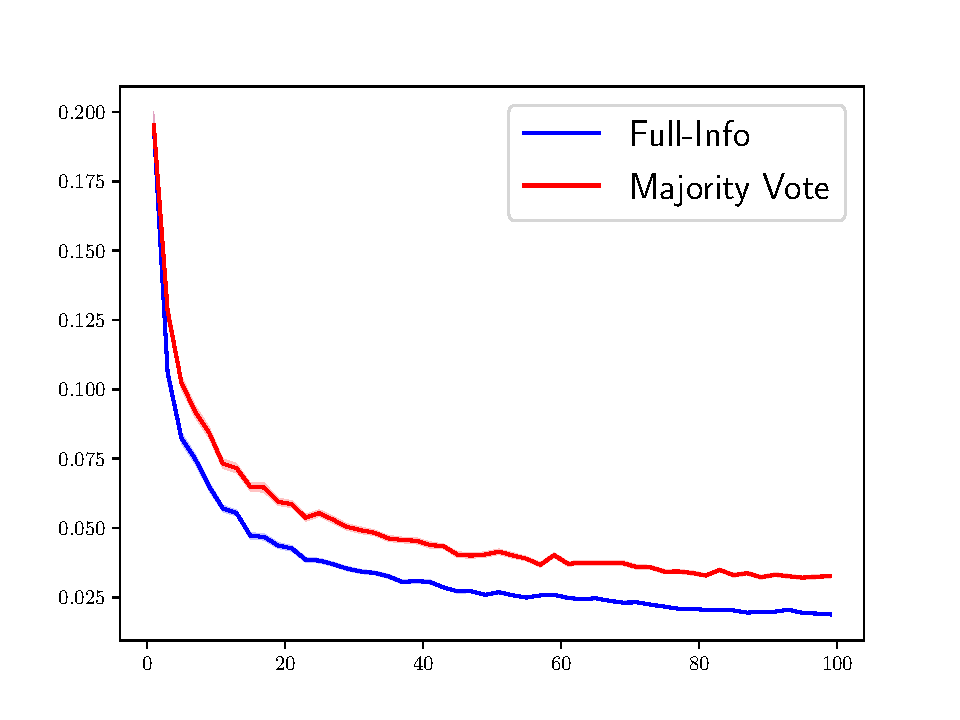
\includegraphics[width=0.3\textwidth]{figure/synthetic-class-05.pdf} &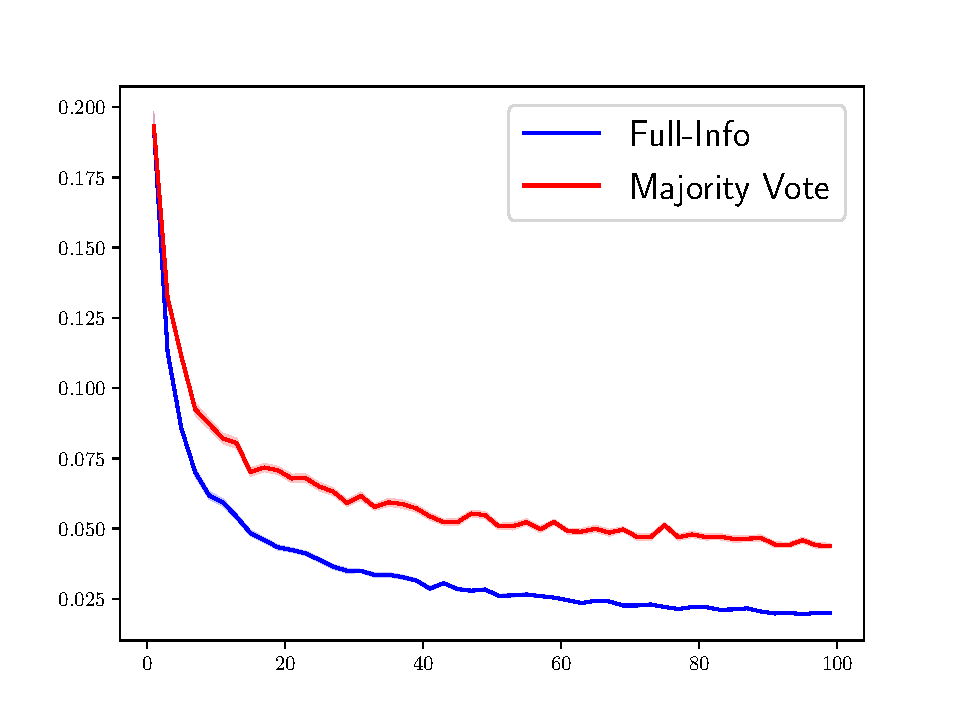
\includegraphics[width=0.3\textwidth]{figure/synthetic-class-10.pdf} &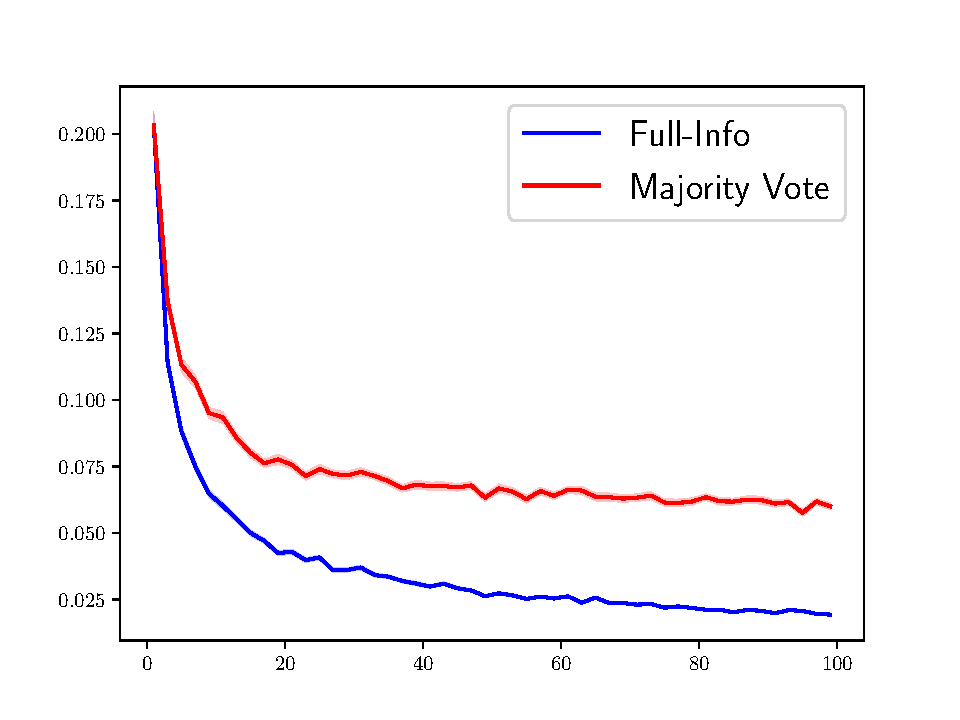
\includegraphics[width=0.3\textwidth]{figure/synthetic-class-15.pdf} \\
%% %		(a) & (b) & (c) \\
%% %		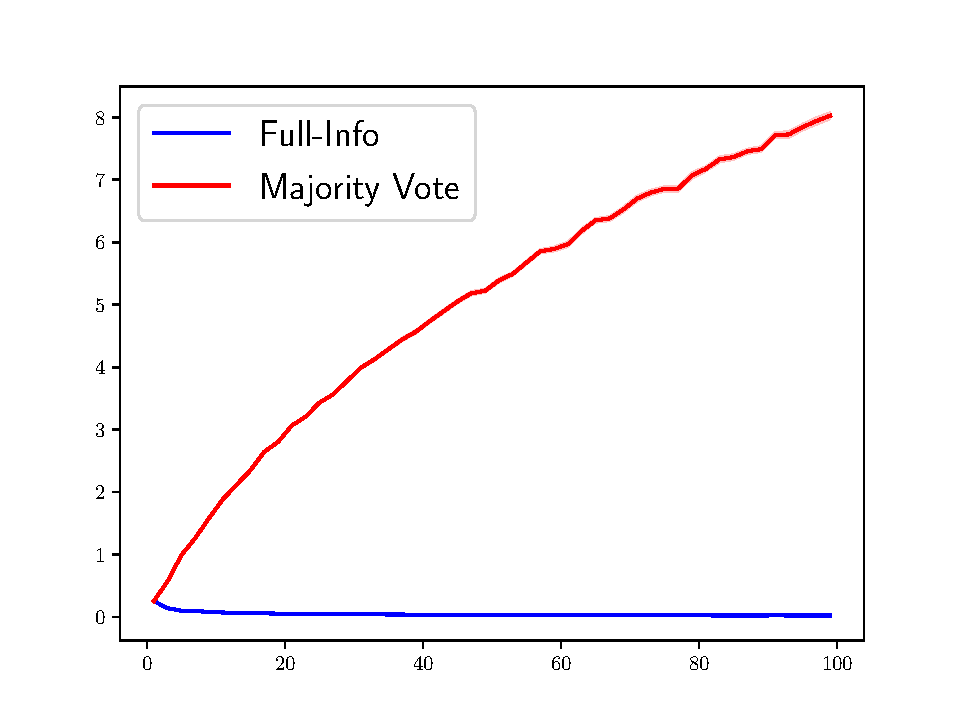
\includegraphics[width=0.3\textwidth]{figure/synthetic-calib-05.pdf} & 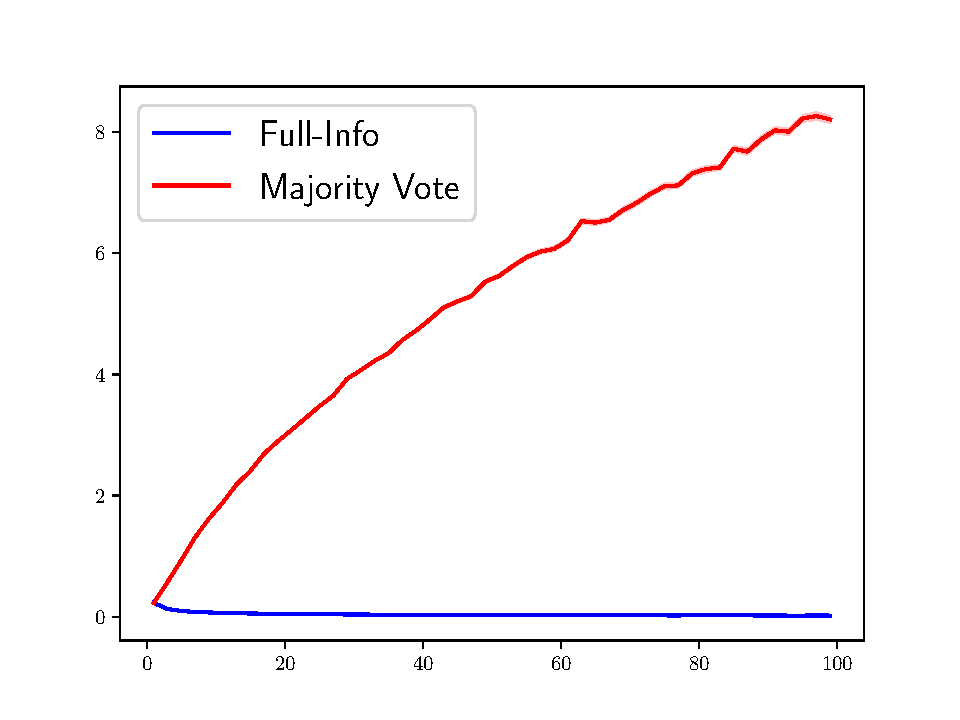
\includegraphics[width=0.3\textwidth]{figure/synthetic-calib-10.pdf} & 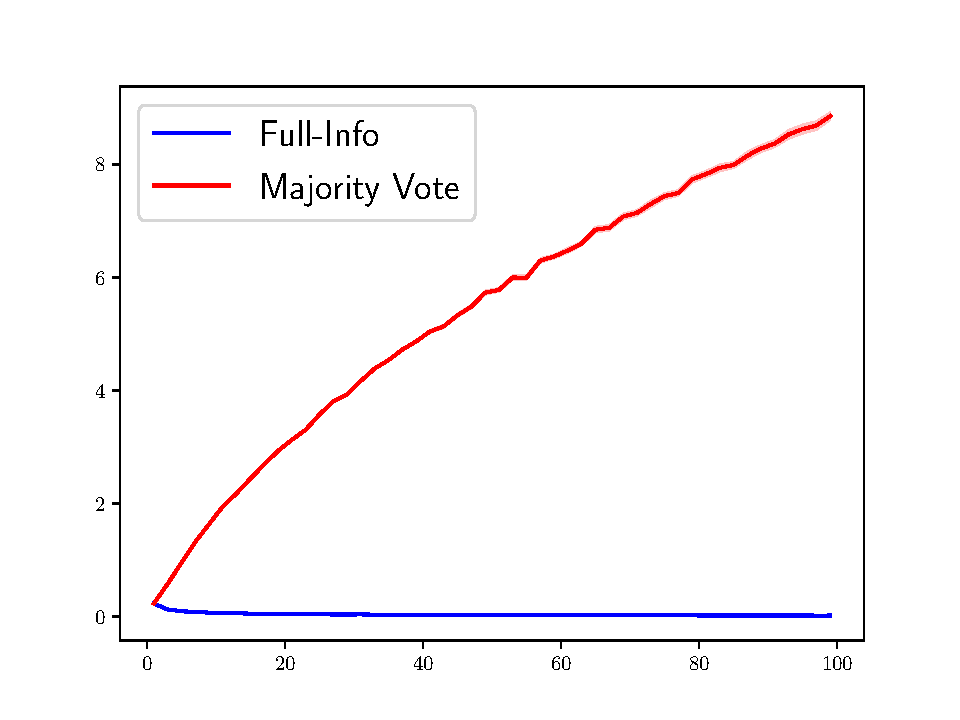
\includegraphics[width=0.3\textwidth]{figure/synthetic-calib-15.pdf}\\
%% %		(a) & (b) &  (c)
%% %	\end{tabular}
%% %	\caption{Classification error and calibration error for synthetic data for $n=1,000$ and $d=10$. For (a) $\beta = 0.5$; For (b) $\beta = 1$; For (c) $\beta = 1.5$. The errors are averaged over 100 trials with 95\% confidence bands.} \label{fig:synthetic}
%% %\end{figure}\ha{can we have only one legend in the plot?}



\subsection{BlueBirds}
\label{sec:BB}

We begin with the
\href{https://github.com/eaplatanios/noisy-labels}{BlueBirds}
dataset~\cite{WelinderBrPeBe10}, a small dataset of 108 images with ResNet features.  The task is to classify each image as one of
\textit{Indigo Bunting} or \textit{Blue Grosbeak} (two similar-looking blue
bird species). For each image, we have $39$ labels, obtained through Amazon
Mechanical Turk workers.  We use an ImageNet pretrained
ResNet50 model to generate image
features, applying PCA to reduce the dimensionality from
$d_{\textup{init}} = 2048$ to $d=25$.

We repeat the following experiment $T = 100$ times.
%
For each number $m = 1, \ldots, 35$ of labelers, we fit
the multi-label logistic model~\eqref{eq:maximum-likelihood}
and the majority vote estimator~\eqref{eq:logistic-majority},
finding calibration and classification errors using 10-fold cross validation.
%
We measure calibration error on an example $x$
by $|\logit(\wt{p}(x)) -
\logit(\what{p}(x))|$, where $\wt{p}(x)$ is the predicted probability,
$\what{p}(x)$ the empirical labeler probability,
and $\logit(p) = \log\frac{p}{1 - p}$; we measure classification
error on example $x$ with
labels $(y_1, \ldots, y_m)$ by $\frac{1}{m} \sum_{j = 1}^m \ind\{y_j \neq
\sgn(\wt{p}(x) - \half)\}$, giving an inherent noise floor because
of labeler uncertainty. We
report the results in Figure~\ref{fig:bluebird}.
These plots corroborate
our theoretical predictions: as the number of labelers $m$ increases, both
the majority vote method and the full label method exhibit improved
classification error, but considering all labels gives a (significant)
improvement in accuracy and in calibration error.

%we train the last layer of a pre-trained model \ha{which dataset for pretraining?} using the two algorithms of interest.
%
%
% \ha{why} and the images are noisy \ha{what does that mean?}.
%For each image
%The dataset was constructed by labels of 39 Amazon MTurk workers, with each of them labeling every image \textit{Indigo Bunting} or \textit{Blue Grosbeak}. For each image $i$, we generate their features $x_i \in \R^d$ by first taking the last layer outputs of a pretrained neural network $\tilde{x}_i \in \R^D$ and using PCA to reduce $\begin{bmatrix} \tilde{x}_1 & \cdots & \tilde{x}_n \end{bmatrix}^\top \in \R^{n \times D}$ to $\begin{bmatrix} x_1 & \cdots & x_n \end{bmatrix}^\top \in \R^{n \times d}$. The plots are shown in Fig.~\ref{fig:bluebird}.



\begin{figure}[ht]
  %% \vspace{-.6cm}
  \begin{center}
    \begin{tabular}{cc}
      \begin{overpic}[width=.48\columnwidth]{%,grid]{%
	  figure/resnet-class-bluebirds.pdf}
	\put(30,-1){{\small Number of labelers $m$}}
	\put(-3,20){
	  \rotatebox{90}{{\small Classification error}}}
      \end{overpic} &
      \hspace{-.3cm}
      \begin{overpic}[width=.48\columnwidth]{%,grid]{%
	  figure/resnet-calib-bluebirds.pdf}
	\put(30,-1){{\small Number of labelers $m$}}
	\put(-3,20){
	  \rotatebox{90}{{\small Calibration error}}}
      \end{overpic} \\
      (a) & (b)
    \end{tabular}
    \caption{\label{fig:bluebird} Experiments on BlueBirds dataset. (a)
      Classification error.  (b) Calibration error $|\logit(\wt{p}) -
      \logit(p)|$ with ResNet features reduced via PCA to dimension
      $d=25$. Error bars show 2 standard error confidence
      bands over $T = 100$ trials.}
  \end{center}
\end{figure}



\subsection{Crowdsourcing methods on semisynthetic CIFAR-10 labels}
\label{sec:semi-synthetic}


\newcommand{\softmax}{\textup{softmax}}

We adapt the original
CIFAR-10 dataset~\cite{KrizhevskyHi09}, which consists of 6000 $32 \times
32$ images from each of $k = 10$ classes (60,000 total images).
%
To mimic collecting messy data, rather than the single-label
in the base CIFAR-10 data, we construct pseudo-labelers
using a pretrained eighteen layer residual network
$f: \mc{X} \to \R^k$ (ResNet18~\cite{HeZhReSu16}) whose accuracy we can
adjust.
%
For $s \in \R^k$, define $\softmax(s) = [e^{s_y} /
  \sum_{l = 1}^k e^{s_l}]_{y = 1}^k$.
%
Then for an input $x \in \mc{X}$, the model outputs a score $f(x)
= {\Theta\opt}^\top \phi(x) \in \R^k$, where
$\Theta\opt = [\theta_1\opt ~ \cdots ~ \theta_k\opt] \in \R^{d \times k}$
is a matrix of per-class weights and
$\phi : \mc{X} \to \R^d$ represents the second-to-last layer
outputs of the neural network.
%
%% \in
%% \R^k$, where $\softmax(f(x))$ indicates the probabilities $\P(Y = y \mid X =
%% x)$.  The model $f$ has the form
%% \begin{equation*}
%%   f(x) = {\Theta\opt}^\top \phi(x), \qquad \text{s.t. }\Theta\opt = [\theta\opt_1 ~ \cdots ~ \theta\opt_k] \in \R^{d \times
%%   	k},
%% \end{equation*}
%% where $\Theta\opt$ is a matrix of per-class weights, and $\phi : \mc{X} \to \R^d$
%% represents the second-to-last layer outputs of the neural network. 
%
As we fit linear models, we take the outputs $\phi(x_i)$ as data, so
$X_i = \phi(x_i)$ are the covariates for the $i$th image $x_i$,
and $\Theta\opt$
is the ground-truth parameter.  We construct labels $Y_{ij}
\in \{1, \ldots, k\}$, $j = 1, \ldots, m$
by choosing the constant $\alpha > 0$
to model labeler expertise, drawing
\begin{equation*}
  \P(Y_{ij} = y \mid X_i = x)
  = \softmax(\alpha f(x))_y
  %% = \softmax(\alpha {\Theta\opt}^\top \phi(x))_y
  = \frac{\exp(\alpha \<\theta\opt_y, \phi(x)\>)}{
    \sum_{l = 1}^k \exp(\alpha \<\theta\opt_l, \phi(x)\>)}.
\end{equation*}
We vary $\alpha$ in experiments to adjust that the median value
of $p_i \defeq \max_{y \in [m]} \softmax(\alpha f(x_i))_y$, where
$p_i \in (1/k, 1)$. In the ``expert labelers'' case, we take
$\alpha \to \infty$ so that $\mbox{median}(\{p_i\}) \to 1$,
while the ``crowd labelers'' case corresponds to
$\alpha \downarrow 0$ and $\mbox{median}(\{p_i\}) \to 1/k$.

We fit $\mve$ and
$\what{\theta}^{\textup{mle}}_{n,m}$ using the multiclass logistic loss.
%
To test our predictions, we also investigate the standard
Dawid-Skene (DS)~\cite{DawidSk79} and GLAD~\cite{WhitehillWuBeMoRu09}
crowdsourcing methods.
%
The DS method models the probability that labeler $j$ assigns label $y'$
given correct label $y$ through a matrix $\alpha_j \in \R^{k \times k}$ with
$p_j(y' \mid y) = \frac{1}{1 + e^{-\alpha_j(y', y)}}$, while GLAD estimates
the probability that labeler $j$ correctly identifies the label of an
example $i$ via $p_{ij} = \frac{1}{1 + e^{-\beta_i \alpha_j}}$, where
$\alpha_j \in [-\infty,\infty]$ indicates labeler $j$'s ability and
$\beta_i \in [0, \infty]$ ambiguity in example $i$.
%
Each method uses EM to approximately maximize the likelihood $\prod_{i =
  1}^n \prod_{j = 1}^m \Prb(Y_{ij} \mid \alpha_j, \beta_i)$ (letting
$\beta_i = 1$ for DS) of the observed labels $Y_{ij}$,
initializing $\alpha$ to maximize the likelihood $\prod_{i = 1}^n \prod_{j
  = 1}^m \Prb(Y_{ij} \mid \majY_i, \alpha_j, \beta_i)$ assuming the majority
votes $\majY_i$ are correct and $\beta_i = 1$.
%
Given estimates $\what{\alpha}$ and $\what{\beta}$, one may impute soft
labels $\what{p}_i \in \R_k^+$ for each example $i$, where $\what{p}_{iy}$
indicates the method's estimated probability that example $i$ is of class
$y$, and hard labels $\what{Y}_i = \argmax_y \what{p}_{iy}$.
%
The labels yield  estimators from, respectively, hard and soft labels via
\begin{equation*}
  \what{\theta}_{\textup{h}}
  = \argmin_{\theta_1, \ldots, \theta_k}
  \sum_{i = 1}^n \log\bigg(\sum_{l = 1}^k
  e^{\<X_i, \theta_l - \theta_{\what{Y}_i}\>}\bigg)
  % \exp(\<X_i, \theta_l - \theta_{\what{Y}_i})\right)
  ~~ \mbox{and} ~~
  \what{\theta}_{\textup{s}}
  = \argmin_{\theta_1, \ldots, \theta_k}
  \sum_{i = 1}^n
  \sum_{y = 1}^k
  \what{p}_{iy} \log\bigg(\sum_{l = 1}^k
  e^{\<X_i, \theta_l - \theta_y\>} \bigg).
  % \exp(\<X_i, \theta_l - \theta_y\>\right),
\end{equation*}
We let $\dse$
and $\glade$ denote the corresponding estimators using hard labels,
and $\dspe$ and $\gladpe$ those trained with the estimated
probabilities $\what{p}_i$.
%
Our experiments use
Crowd-Kit~\citep{UstalovPaTs24}.

\begin{figure}[ht]
  %% \vspace{-.6cm}
  \begin{center}
    \begin{tabular}{cc}
      \hspace{-2cm}
      \begin{overpic}[width=.65\columnwidth]{%,grid]{%
	  figure/hard-test-error.pdf}
      \end{overpic} &
      \hspace{-2.5cm}
      \begin{overpic}[width=.65\columnwidth]{%,grid]{%
	 figure/soft-test-error.pdf}
      \end{overpic} \\
      \hspace{-2cm} (a) &
      \hspace{-2.5cm} (b) \\
      \hspace{-2cm}
      \begin{overpic}[width=.5\columnwidth]{%,grid]{%
	  figure/105.pdf}
      \end{overpic} &
      \hspace{-2.5cm}
      \begin{overpic}[width=.5\columnwidth]{%,grid]{%
	  figure/42.pdf}
      \end{overpic} \\
      \hspace{-2cm} (c) & \hspace{-2.5cm} (d)
    \end{tabular}
    \caption{\label{fig:semisynthetic} Experiments on semisynthetic
      CIFAR-10 dataset. Median labeler accuracy represents the
      median of $p_i = \max_y \softmax(\alpha f(x_i))_y$
      on the training data. Results are
      averaged over $20$ trials, and vertical axes
      give mis-classification rate from (synthetic) ground-truth labels
      on held-out test set. Legend keys correspond to
      maximum likelihood $\what{\theta}^{\textup{mle}}_{n,m}$ (MLE),
      majority vote $\mve$ (MV), hard-labeled Dawid-Skene (DS) and
      GLAD crowdsourced estimators $\dse$ and $\glade$,
      and soft-labaled Dawid-Skene (DS prob) and GLAD (GLAD prob)
      estimators $\dspe$ and $\gladpe$.
      (a) Comparison of methods using hard labels.
      (b) Comparison with crowdsourced estimated soft-labels.
      (c) Number of labelers $m$ versus test error for
      median accuracy $p = .105$ (noisy labelers). (d)
      Number of labelers $m$ versus test error for
      median accuracy $p = .4$. Both (c) and (d) report
      95\% error bars over the trials.}
  \end{center}
\end{figure}

We report the results in Fig.~\ref{fig:semisynthetic}. As we see,
when the model is well-specified,
the MLE $\what{\theta}^{\textup{mle}}_{n,m}$ %%with soft labels 
outperforms aggregation methods and black-box crowdsourcing models that
generate soft labels. Crowdsourced $\dse$ and
$\glade$ yield smaller test error than $\mve$, and using the soft labels,
$\dspe$ and $\gladpe$ further reduces the error, suggesting benefits
to using soft labels from crowdsourcing for training even if the
underlying model is unknown.
